\chapter{M-LWE Comparison and Evaluation}

\unsure[inline]{should i add a precious chapter with implementation details, describe this in an sunsection here briefly or leave it completely out?}

In this chapter the three different LWE Schemas (Plain-LWE, R-LWE and M-LWE) will be first evaluated on there own and in comparison.

\section{Output size comparison}

The initial comparison will be the size in bits of the various output variables generated when working with the different schemes. The output is dependent on four variables: the matrix dimension $n$, the polynomial rank $d$, the number of bits of the modulus $q_b$ and the number of bits of the message $\ell$. In the case of Plain-LWE, the polynomial rank is equal to one, while in R-LWE, the matrix dimension is equal to one. In all other cases, the polynomial rank and matrix dimension are greater than one. The size of the different variables can be calculated based on the dimensions defined in Table \ref{table:LweKeys}. As the $rlk$ is essentially a modified private key, it has the same dimension; it is simply required $n$ times. All equations for computing the number of bits needed for the different variables for the schemes can be found in Table \ref{table:OutputVariableSize}. 

\begin{table}[h]
  \centering
  \caption{LWE output variable size in bits based on $n$, $d$, $q_b$ and $\ell$}
  \begin{tabular}{|l|c|c|c|}
    \toprule
          & Plain-LWE                       & R-LWE                                                        & M-LWE                                                               \\
    \midrule
    $sk$  & $n \cdot q_b$                   & $d \cdot q_b$                                                & $n \cdot d \cdot q_b$                                               \\
    $pk$  & $(n^2 +n) \cdot q_b$            & $2 \cdot (d \cdot q_b)$                                      & $(n^2 + n)\cdot d \cdot q_b$                                        \\
    $rlk$ & $n \cdot ((n^2 +n) \cdot q_b)$  & $2 \cdot (d \cdot q_b)$                                      & $n \cdot ((n^2 + n)\cdot d \cdot q_b)$                              \\
    $m$   & $\ell$                          & $\left\lceil \ell/d \right\rceil \cdot d$                    & $\left\lceil \ell/d \right\rceil \cdot d$                           \\
    $ct$  & $\ell \cdot((n + 1) \cdot q_b)$ & $\left\lceil \ell/d \right\rceil \cdot(2 \cdot d \cdot q_b)$ & $\left\lceil \ell/d \right\rceil \cdot ((n + 1) \cdot d \cdot q_b)$ \\
    \bottomrule
    
  \end{tabular}
  \label{table:OutputVariableSize}
\end{table}

To provide a more intuitive understanding of the differences between the various schemes, a simulation of the values can be observed in Figure \ref{fig:OutputFactors}. The development of the number of factors is plotted for the different schemas based on $n$ and $d$. The number of factors is equivalent to the equations in Table \ref{table:OutputVariableSize} if $q_b=1$. This is equivalent to the number of factors that need to be stored for the output variable. If a larger modulus is used, the number of factors can be multiplied by it, thereby determining the total number of storage in bits that is required. For $m$ and $ct$ a value of $l=64$ was chosen, to reflect different properties. In the case of P-LWE, the matrix dimension, $n$, is plotted against the number of factors. In contrast, for R-LWE, the polynomial rank, $d$, is plotted against the number of factors. Given that M-LWE relies on two variables, namely $n$ and $d$, it was decided that the best approach would be to plot $n$ against the number of factors, with multiple lines representing different values of $d$. This was done to simplify the visualization of the differences, as a three-dimensional plot is more challenging to comprehend, particularly when printed in two dimensions. Additionally, the value of $d$ is always linear in relation to the number of factors, indicating that it solely affects the slope of the change in $n$, as evidenced in the plot.


\begin{figure}[ht!]
  \centering
  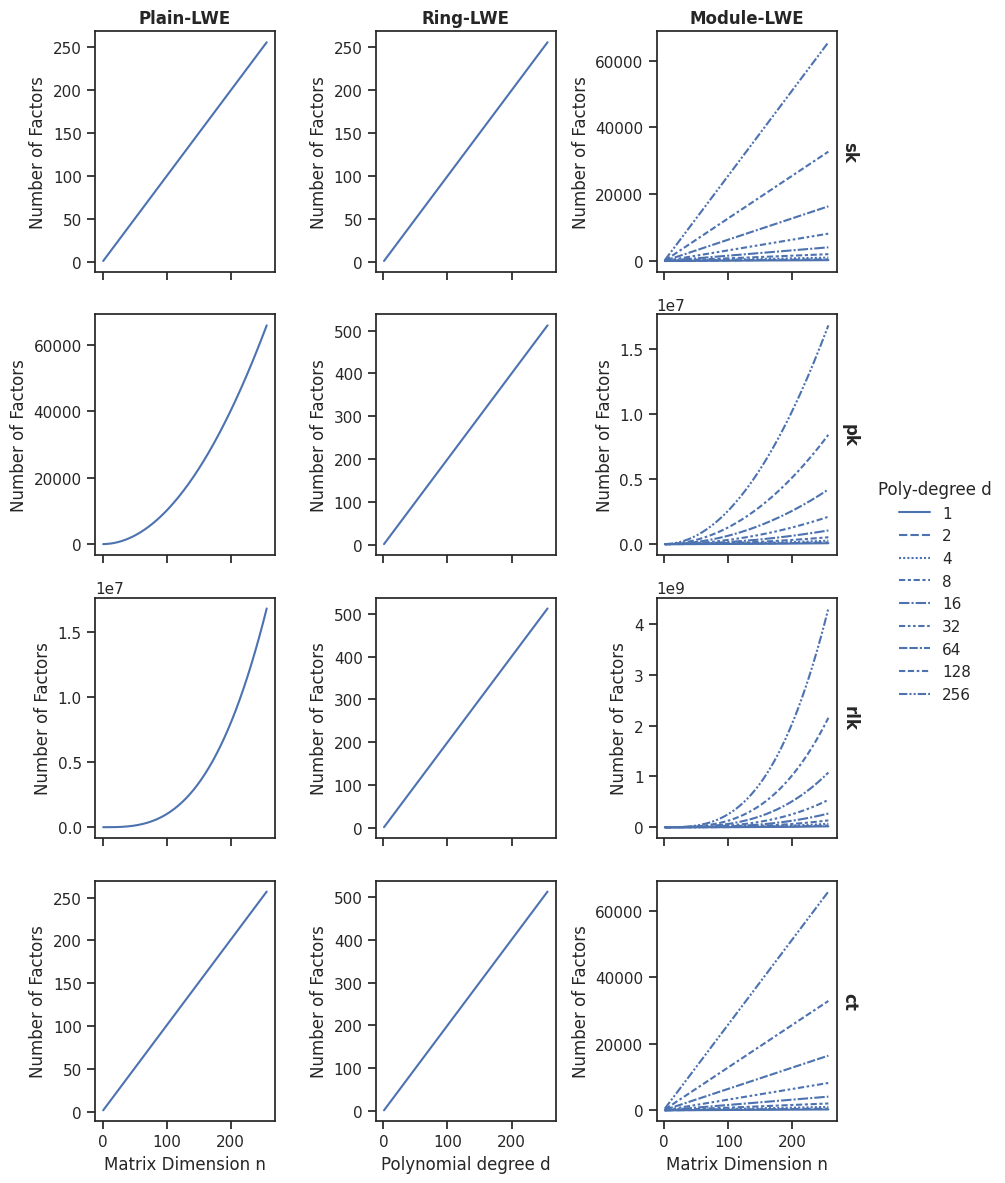
\includegraphics[scale=0.55]{images/OutputFactors.png}
  \caption[Output Variable Factors by Scheme]{The development of factors for the various output variables by schema, based on $n$ and $d$. In the case of M-LWE, the different line types indicate different values of $d$. The message length $l=64$}
  \label{fig:OutputFactors}
\end{figure}

The growth rates observed for the secret key $sk$ are linear with regard to the variables $n$ and $d$ for Plain-LWE and R-LWE, respectively. In contrast, M-LWE exhibits a linear relationship with either $n$ or $d$. When both variables grow simultaneously, the growth rate becomes quadratic. As a consequence, the growth rate for the number of factors in this case exhibits a significantly higher rate of increase than that observed for the other two schemes.

The linear growth rate observed for R-LWE remains constant for both the private key $pk$ and the relinearization key $rlk$. In contrast, the growth rates for the other two schemes exhibit a significant increase, particularly with regard to the matrix dimension $n$. For $pk$, the growth rate is quadratic, while for $rlk$, it is even cubic. When increasing the polynomial rank simultaneously, the growth rate for M-LWE becomes cubic or quartic, respectively.

It should be noted that there is a slight caveat associated with the message and the ciphertext in the context of R-LWE and M-LWE. Due to their simultaneous encryption of multiple bits, there is a possibility of either over- or undershooting the necessary amount. This phenomenon can be observed in the plots for the output variables $m$ and $ct$, with the message length $l$ set to $64$ bits. In contrast to L-LWE, where the number of factors for $m$ is constant, as each bit is treated separately, the number of factors needed for R-LWE and M-LWE depends on the polynomial rank $d$. In the event that the length of the message, denoted by $l$, exceeds the degree of the polynomial, it is necessary to create a multitude of polynomials of degree $d$ in order to encrypt the entire message. If the length of the message, represented by $l$, is not evenly divisible by the polynomial rank, $d$, an additional polynomial must be created and padded. Conversely, if the length of the message is smaller than the polynomial rank, the message will fit into one polynomial, but the extra size must be padded. This is why the number of factors initially remains at 64 and then begins to increase, as the polynomial is too large for the message, resulting in wasted space.

Apart from this, the scaling of the number of factors is linear with respect to the dimension variables, namely $n$ and $d$. Consequently, for R-LWE, the number of factors is identical to that of the private key $pk$ and the relinearization key $rlk$ when $d$ is equal to or greater than $l$. In all other cases, the number of factors is a multiple of this value, dependent on the number of polynomials that must be created to fit the message. In the case of M-LWE and Plain-LWE, the number of factors is comparable to that of the secret key, $sk$. However, in the case of M-LWE, a similar situation arises with R-LWE, whereby the number of factors required can be a multiple based on the size of $d$. In the case of Plain-LWE, the increase is significantly more pronounced, as each bit must be encrypted individually, resulting in the generation of a distinct ciphertext for every bit.

In general, R-LWE requires the fewest number of factors and the smallest amount of physical space to store its output variables. In comparison, Plain and especially M-LWE require a greater number of factors and a greater amount of physical space. Furthermore, the growth rate for R-LWE is significantly lower than that of Plain and M-LWE. In defense of M-LWE, it should be noted that in practice the matrix dimension $n$ is quite small. In the CRYSTALS-Kyber scheme \cite{CyrstalsKyber}, the values are set between 2, which corresponds to low security, and 4, which corresponds to high security. This can be achieved because the security of the system is not solely dependent on the matrix, but also on the polynomials. In contrast to Plain-LWE, significantly larger values of $n$ are required for security. In the Frodo encryption scheme \cite{frodo}, which utilize Plain-LWE, values between $352$ for low security and $864$ for high security and a value of $n=752$ is recommended. This results in the number of factors exceeding $400$ million just for the $rlk$.

A comparison of the physical space required for the various encryption schemes, with variables based on the regular/recommended security level of published encryption schemes that employ the underlying method, can be found in Table \ref{table:OutputVariableInKB}. It is important to note that the results should be interpreted with caution and that direct comparisons between the numbers are not possible. However, the data provides a general indication of the differences between the schemes. Notably, the variables for Plain-LWE are considerably larger than those for the other two, requiring nearly 800 megabytes, solely for the RLK. Even when the ciphertext $ct$ is the smallest, this amount of disk space is necessary for each bit, whereas R-LWE and M-LWE can store 512 or 256 bits, respectively, with a slightly larger $ct$. With the exception of the ciphertext, R-LWE has the smallest overall size for every variable. However, as it can store twice the information of M-LWE and, as previously mentioned, 512 times more than Plain-LWE, it requires the smallest amount per bit stored.

\begin{table}[h]
  \centering
  \caption{LWE Output Variable size in Kilobyte (KB), based on variables for the regular/recommended security level of published encryption schemes}
  \begin{tabular}{|l|c||c|c|c|c||c|c|c|c|}
    \toprule
              & Source                      & $n$   & $d$   & $q$      & $q_b$ & $sk$    & $pk$      & $rlk$    & $ct$    \\
    \midrule
    Plain-LWE & \cite{frodo}                & $752$ &       & $32767$ & $15$  & $1.41$  & $1061.73$ & $798421$ & $1.412$ \\
    R-LWE     & \cite{PracticalKeyExchange} &       & $512$ & $25.601$ & $15$  & $0.96$  & $1.92$    & $1.92$   & $1.92$  \\
    M-LWE     & \cite{CyrstalsKyber}        & $3$   & $256$ & $7681$   & $13$  & $1.248$ & $4.992$   & $14.976$ & $1.664$ \\
    \bottomrule
  \end{tabular}
  \label{table:OutputVariableInKB}
\end{table}

In conclusion, the comparison based on the size of the output values indicates that R-LWE has the slowest growth of physical space needed based on its dimension variables. Although M-LWE has the fastest growth rate, as it is based on multiple dimension variables, this makes it far more secure than Plain-LWE. Consequently, the dimensions can be smaller in general to achieve a similar level of security, which results in a smaller physical size of its output variables. In terms of storage requirements for the output variables, Plain-LWE is by far the most demanding, with M-LWE requiring more physical space than R-LWE. However, the difference in these requirements is not as significant as that observed in the comparison with Plain-LWE.